\chapter{人工智能基础（吴琳鑫）}

\section{人工智能、机器学习、深度学习的关系}

人工智能（AI）是一个涵盖广泛且深刻的学科，旨在通过模拟和实现人类智能的各种特征，使机器能够执行通常需要人类智慧的任务。AI的应用范围广泛，从语言理解、图像识别到复杂的决策制定，几乎渗透到我们生活的每一个角落。AI的核心目标是创造能够感知、理解、推理、决策以及学习的智能系统，这一目标推动着科技的不断进步。随着技术的发展，AI已经在医疗、金融、交通、娱乐等多个领域发挥着重要作用，成为推动社会和经济变革的关键力量。

AI的发展历程可以分为多个阶段。最初，人工智能系统依赖于规则和符号推理，这些系统基于人为设定的规则来模拟人类的推理过程。然而，这种基于规则的方法在处理复杂和不确定的情况时显得力不从心，无法适应现实世界中的多变环境。为了克服这些限制，AI的发展逐渐转向数据驱动的机器学习（Machine Learning, ML）。

机器学习强调通过大量数据的训练，让计算机系统自主发现数据中的规律和模式，从而做出更智能的预测和决策。与传统的基于规则的方法不同，机器学习无需人工编写所有的规则和逻辑，而是通过算法自动从数据中提取有用的信息。这一方法的出现使得AI能够应对更加复杂和动态的任务，特别是那些难以通过人工规则描述的任务。例如，机器学习在自然语言处理、图像分类和推荐系统等领域取得了显著成果，极大地提升了AI系统的智能化水平。

机器学习的基本思想可以归纳为“数据驱动”。在这种框架下，模型通过分析输入数据进行训练，逐步优化模型参数，以便在遇到新数据时能够做出更准确的预测或分类。机器学习的方法多种多样，主要包括监督学习、无监督学习和强化学习等，每种方法适用于不同类型的任务。在监督学习中，模型通过学习带有标签的数据，掌握输入与输出之间的关系；无监督学习则侧重于从未标注的数据中发现潜在的结构和模式，常用于数据的聚类和降维；强化学习则模拟智能体在与环境互动中学习最优策略，广泛应用于游戏和机器人控制等领域。尽管机器学习在许多领域取得了令人瞩目的成果，但它仍面临一些挑战，如对大量标注数据的依赖以及模型“黑箱”问题，即决策过程难以解释和理解，这在高风险领域（如医疗和金融）尤为重要。

深度学习（Deep Learning, DL）是机器学习的一个重要分支，特别注重通过模仿人脑神经网络的结构和功能来进行学习。深度学习的主要优势在于其强大的自动特征提取能力。通过多层神经网络，深度学习能够对输入数据进行逐层处理，自动提取出不同层次的特征表示，从而实现高效的模式识别。与传统机器学习方法相比，深度学习的最大特点是无需手工提取特征，能够自动从数据中学习复杂的特征表示，这使得深度学习在处理图像、语音和文本等复杂数据时表现尤为出色。

深度学习的成功离不开现代计算能力的提升，尤其是图形处理单元（GPU）的普及，大大加速了大规模神经网络的训练过程。深度学习已经在多个领域取得了革命性的进展。例如，在图像识别领域，卷积神经网络（Convolutional Neural Network, CNN）能够自动提取图像中的边缘、纹理和形状等关键信息，被广泛应用于人脸识别和自动驾驶等任务。在自然语言处理领域，循环神经网络（Recurrent Neural Network, RNN）和长短期记忆网络（Long Short-Term Memory, LSTM）能够有效处理序列数据，应用于机器翻译和情感分析等任务。深度学习通过其在自动特征学习和非线性建模上的优势，常常在处理高度复杂和非线性的问题时，超越传统机器学习方法。尽管深度学习在许多领域展现了强大的能力，其发展也面临一些挑战。首先，训练深度神经网络需要大量的计算资源和存储空间，这对于资源有限的环境来说是一大障碍。其次，深度学习模型的“黑箱”性质使得其决策过程难以解释，这在某些需要高可解释性的应用场景中（如医疗诊断和金融风控）带来了不确定性和风险。此外，深度学习模型通常需要大量的高质量数据进行训练，而在数据获取和标注困难的领域，模型的训练效果可能受到限制。

总的来说，人工智能、机器学习和深度学习三者之间存在着紧密的关系。人工智能是一个广泛的领域，涵盖了各种模拟和实现人类智能的技术和方法；机器学习作为实现人工智能的重要手段，通过数据驱动的方法让计算机系统自主学习和改进；而深度学习则是机器学习的一个强大分支，通过多层神经网络实现更为复杂和精确的模式识别和决策制定。

随着科技的不断进步，人工智能、机器学习和深度学习将继续相互促进，共同推动智能系统的发展和应用。接下来，我们将深入探讨机器学习和深度学习的核心概念、方法以及它们在实际应用中的具体表现，以全面理解这一领域的最新进展与未来趋势。

\section{机器学习}

人工智能、机器学习和深度学习的关系体现了技术发展的层级性，如图\ref{fig:人工智能、机器学习和深度学习的关系}所示。人工智能的目标是让机器具备与人类相似的智能能力，机器学习则是实现这一目标的一种重要方法，专注于从数据中学习和发现规律。深度学习作为机器学习的一个子领域，进一步提升了数据处理的深度和复杂性，能够解决许多传统方法无法处理的难题。随着深度学习技术的成熟和应用，人工智能在许多领域正迎来前所未有的突破，尤其是在处理复杂任务和大规模数据时，深度学习已成为推动AI发展的核心动力。

\begin{figure}[H]
    \centering
    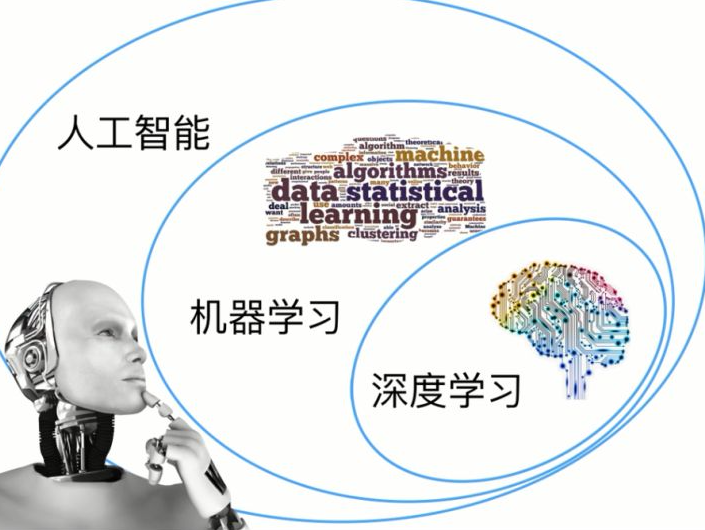
\includegraphics[width=0.7\linewidth]{image/2/人工智能、机器学习和深度学习的关系.png}
    \caption{人工智能、机器学习和深度学习的关系}
    \label{fig:人工智能、机器学习和深度学习的关系}
\end{figure}

在前面的章节中，我们探讨了人工智能（AI）如何进行精准的判断和预测。接下来，我们将深入了解实现这些能力的关键方法——机器学习。作为推动人工智能发展的核心技术，机器学习让计算机能够通过大量的数据自主学习和不断改进，而无需人为制定详细的规则。简单来说，机器学习就像是在教会计算机通过观察和分析大量的信息，自行发现其中的规律，并据此做出智能决策。

机器学习的魅力在于它的自适应能力。传统的编程方式需要开发者为每一个可能的情况编写具体的指令，这在面对复杂和多变的问题时显得力不从心。而机器学习通过让计算机从数据中学习，不断调整和优化其算法，使其能够应对各种复杂的任务和环境。这种方法不仅提高了效率，还极大地拓展了AI的应用范围，从图像和语音识别到自然语言处理和自动驾驶，机器学习无处不在，成为现代科技发展的重要驱动力。

通过机器学习，AI能够不断进步，适应新的挑战和需求。这种持续学习和自我优化的能力，使得AI不仅能够解决当前的问题，还能预见和应对未来的变化。接下来的小节，我们将以机器学习的定义、原理、分类和学习方式与评估为重点，深入探讨这一关键技术是如何赋予AI强大智能的。

\subsection{机器学习的定义}

当我们回顾日常生活，会发现自己其实常常依靠“经验”来解决各种问题：小时候，通过反复尝试拼搭不同形状的积木，我们逐渐找到了能够搭建更稳固房屋的方法；长大后，通过观察老司机是如何控制方向和车速，借由不断的上路练习，我们最终熟练掌握了驾驶技巧。这些过程并不需要别人从头到尾、按部就班地告知我们所有步骤；相反，我们更多依赖的是对环境、事物持续而灵活的感知，从而一点点积累和总结出新的应对策略。

机器学习（Machine Learning）概念的提出，正是把人类这种“经验学习”的模式赋予计算机，使其能够“模仿”人类学习的部分思维过程。在传统编程方法中，我们往往需要事先为计算机设定详细且严格的规则，以处理各种具体场景。然而，很多实际问题并不易通过一条条显式的指令来解决：例如，要让计算机分辨图片中的猫和狗，我们需要面对色彩、姿态、背景杂物等复杂影响因素。此时，与其耗费大量精力去罗列猫狗外观、体型乃至毛发等特征的精确描述，不如直接让计算机“观察”大量带有猫或狗标签的图片，让它通过不断试错和归纳，自动寻找能够区分两者的特征。这样一来，计算机在训练结束后即能在面对新图像时“认出”其中所包含的动物类型，而无需我们再去更新规则或补充新指令。

从这个角度出发，机器学习的核心就是将繁琐的规则制定过程转换为对数据的“经验学习”过程，让计算机可以在大规模、复杂多样的环境中自主识别模式、归纳规律。它强调让计算机通过已有数据加上特定的学习算法，反复迭代和优化自身，从而在新场景下也能做出相对准确、合理的判断或预测。换言之，机器学习并非要为计算机提供现成的答案，而是给予它“学习”的能力，让它在面对全新问题时可以活学活用、举一反三。更进一步说，机器学习所扮演的角色，还在于帮助计算机挖掘数据中潜藏的内在逻辑与关联。当数据规模日益庞大，且维度和结构愈发复杂时，传统的规则式编程常常会力不从心。而机器学习则可以通过分类、回归、聚类、降维等多种方法，对大规模、非线性的混杂数据进行建模和模式识别，并在训练过程中不断修正假设与参数。正是这种基于数据的迭代学习，使得计算机在面临复杂任务时依然能够自适应地调整决策策略，展现出难以想象的灵活度与智能化水平。因此，从本质上讲，机器学习让计算机在没有人类“手把手”指令的情形下，通过对已有数据的自我试验和归纳逐步成长为“智慧型助手”。它不仅能够为我们分担大量重复性、模式化的工作，也在不断冲击和重塑各行各业的技术应用边界。接下来，随着对机器学习内部原理的进一步探讨，我们将看到，计算机究竟如何借助算法与模型，从数据中构建起问题的解题思路，并在实战中持续迭代、不断优化，逐渐变得更加“聪明”。

\subsection{机器学习原理}

想象你是一名刚入门的烘焙学徒。你面前摆满了各种食材与调料（数据），却并不清楚哪些组合能呈现出最佳风味。首先，你会仔细挑选并清洗这些原料，确保没有杂质（数据清洗与整理）。接着，你会琢磨哪些食材最能决定甜点的口感与层次（特征提取与选择）。在选择出关键食材后，你便按照大师传授的配方和技巧（算法与模型）不断尝试烘焙（模型训练），品尝成品的味道来判断是否需要微调用量与火候（模型验证与评估）。如果觉得蛋糕太甜，你会减少糖的用量；如果某种香料毫无贡献，你就不再使用它（模型优化）。通过这样多次尝试与总结经验的过程，当你再次面对全新食材或口味需求时，已经能够轻松应对，并创造出美味的甜点（预测与泛化）。这正是机器学习的基本原理——通过数据驱动的反复试错和经验积累，让模型（学徒）逐渐掌握深藏于数据中的规律与技巧。

从这一类比出发，我们可以更直观地理解机器学习的内部运作机制。计算机就像是一名勤奋的新手烘焙学徒，它的“学习”过程大致包含以下环节：
\begin{enumerate}
    \item \textbf{数据收集与整理}：数据是机器学习的基础材料，就像制作蛋糕前需要精选优质的面粉、奶油和鸡蛋一样。开发者会收集大量资料（图片、文本、声音或数值数据），并对其清洗、整理，确保信息准确完整，为后续步骤打下坚实的基础。
    \item \textbf{特征提取与选择}：并非所有细节都对结果有帮助。就像烘焙中最关键的材料是面粉、黄油和糖，而非烤箱上的花纹和装饰品一样，在机器学习中，我们需要从海量数据中挑出真正影响预测结果的核心特征，确保模型关注真正重要的因素。
    \item\textbf{模型训练}：当有用的特征确定后，模型就像烘焙教程中的配方，它通过不断试验与调整（算法迭代和参数校正）来“理解”数据的规律。比如，初期模型不清楚如何区分猫和狗的照片，但经过多轮试错和反馈后，它会逐渐发现耳朵形状、脸部轮廓等特征更有助于正确判断。
    \item \textbf{验证与评估}：每次完成烘焙后，都需要有人品尝以确保甜点够不够松软、甜度是否适中。同样，机器学习会使用一部分数据进行验证与评估，以确保模型不仅能识别“旧”案例，也能在全新问题面前表现出色。准确率、精确率、召回率等指标正是帮助我们客观衡量模型质量的“味觉尺子”。
    \item \textbf{持续改进}：如果发现蛋糕口感干涩，我们会增加黄油或牛奶的比例。同理，机器学习模型也会根据反馈不断优化参数、尝试新算法，使其在面对新挑战时更为灵活，从而持续提升性能与适用性。
\end{enumerate}

通过这一过程，我们看到机器学习模型如何在数据的指引下“尝试”“反思”与“精进”，最终在复杂的任务中游刃有余。当理解了这一流程，我们便可更清晰地在不同的任务类型和数据条件下，选择恰当的学习方法。接下来，在机器学习的分类部分，我们将探讨不同的学习范式（如监督学习、无监督学习、强化学习和迁移学习）各自的适用场景与特点。

\subsection{机器学习的分类}
在前一小节中，我们通过“烘焙”的类比，了解了机器学习是如何像一位“学徒”一样，通过不断的试错和总结，逐渐掌握技能。就像一个烘焙师傅通过反复调整配方和技巧，最终做出美味的蛋糕，机器学习也通过多次学习和优化，逐步提高模型的表现。不同的学习任务、数据和目标，就像不同的烘焙方式和食材搭配，要求我们采用不同的学习策略。接下来，我们将用“烘焙”的类比来说明机器学习的几种主要分类。

\begin{figure}[H]
    \centering
    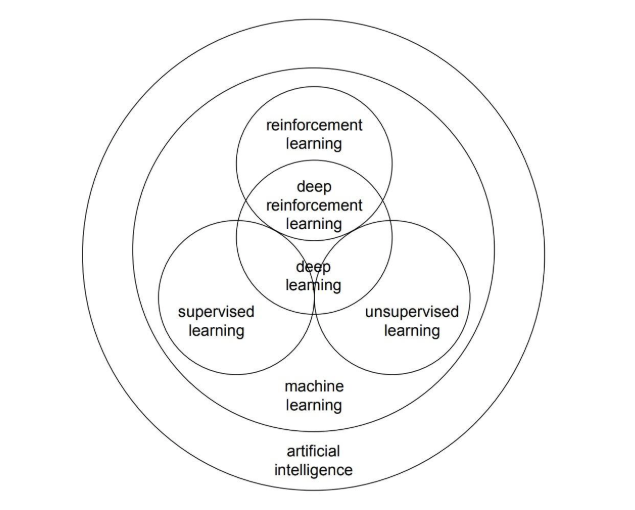
\includegraphics[width=0.8\linewidth]{image/2/分类.png}
    \caption{机器学习的主要分类}
    \label{fig:机器学习的主要分类}
\end{figure}

\begin{itemize}
    \item \textbf{监督学习}: 想象你正在烘焙蛋糕，师傅给你一个详细的食谱，告诉你每一步该如何操作，每个步骤要使用什么食材，结果也早已标定好了——蛋糕的样子、味道和质感。监督学习就像这样，师傅提供了一个明确的指导（即“正确答案”）。你只需按照食谱中的步骤反复操作，直到每次做出来的蛋糕都符合预期的标准。监督学习的关键是模型在训练时，通过已有的标注数据（即食谱）来学习输入和输出之间的关系。每当做错了（比如放错了材料），模型就会调整，从而不断提高自己的“烘焙技巧”。
    \item \textbf{无监督学习}: 有时，烘焙过程中并没有一份具体的食谱，而是你自己通过尝试，逐渐发现哪些食材和搭配能做出美味的蛋糕。无监督学习就像这种情况，模型没有现成的标签来告诉它“应该是怎样的结果”，它只能根据不同的食材和做法去探索，自己总结出哪些搭配效果最好。在无监督学习中，模型试图从数据中找到潜在的结构和模式，就像烘焙师傅自己发现不同口味蛋糕的配方一样。例如，你可能发现，加入适量的杏仁粉的蛋糕总是特别松软，而加入不同的果仁可以创造出独特的口味。这种探索的过程，不依赖于任何标注的答案，模型通过对数据的观察和分析，自己找出规律。
    \item \textbf{强化学习}: 强化学习就像你在烘焙的过程中，自己在厨房里反复尝试，通过不断的实践和反馈逐渐改进。刚开始，你可能不确定哪种温度和时间设置最合适，每一次烘焙后，你会通过品尝蛋糕来判断自己的做法是否正确。如果蛋糕做得太干，你会调整温度和烘焙时间；如果蛋糕太湿，你会改变原料的比例。强化学习的核心是通过试错和反馈（即奖励或惩罚）来优化决策。每次尝试后，模型根据结果（是否成功烘焙出完美的蛋糕）来调整自己的行为，最终学会如何根据环境的变化做出最佳选择。这个过程像是烘焙师傅通过不断的反复练习，从失败中总结经验，最终找到最佳的烘焙方案。
    \item \textbf{迁移学习}: 有时候，烘焙师傅已经掌握了烘焙蛋糕的基本技巧，但他并不需要从头开始学习每个新菜式。假如他已经掌握了如何做巧克力蛋糕，他可以快速地将这些经验迁移到做其他口味的蛋糕上——只需稍微调整一些材料和方法，就能适应新的任务。迁移学习正是这样的过程，模型利用已经学到的知识，帮助自己快速适应新的任务或数据。当你已经熟悉了如何做一个巧克力蛋糕后，做一个香草蛋糕时，你可以借用之前学到的技巧，减少从零开始学习的时间。迁移学习让模型在面对新任务时，能够更快地借用之前的经验和知识，从而加速学习和适应。
\end{itemize}

通过烘焙的类比，我们可以看到，机器学习的不同分类就像烘焙师傅在厨房中采用不同的方法：有时候需要明确的指导（监督学习），有时需要自己探索（无监督学习），有时则通过不断的尝试和反馈来改进技巧（强化学习），而有时则能通过借用已有经验来加速学习（迁移学习）。每种方法都有其独特的优势和适用场景，在实际应用中，我们往往需要根据具体的任务和数据，选择最合适的学习方式，以便做出最完美的“蛋糕”——即解决方案。当然，选择合适的学习方式只是第一步。就像一个烘焙师傅不仅要掌握不同的做法，还需要通过不断品尝和调整来确保每次烘焙都能达到理想的效果，机器学习模型的学习过程也需要通过合适的评估来指导和优化。在接下来的小节中，我们将探讨如何评估模型的学习效果，确保我们选择的“烘焙”方法能够最终做出符合预期的“蛋糕”。

\subsection{机器学习的学习方式、评估与优化}

当你学会做一道菜时，你不只是机械地记住菜谱，还会反复尝试、调整味道，直到自己觉得满意为止。机器学习的过程与此类似：模型需要反复“品尝”数据的滋味，微调“调料”比例，直到在面对新食材（数据）时，仍然能做出可口的料理（预测或决策）。这一过程不仅是对数据的反复“阅读”，更是一次次的优化和调整。

机器学习的学习过程通常分为几个阶段：训练、预测、评估和优化。每一个阶段都像是在做菜过程中不断调整和完善的步骤。首先是训练阶段，就像是学厨的新手反复练习，模型会多次“阅读”大量已知结果的数据（训练集），通过调整模型的参数来理解数据中的内在规律。例如，烤蛋糕的温度、时间和配料比例，你会不断调整，直到找出合适的配方。在机器学习中，数据的质量和数量直接影响到模型的学习效果。良好的数据帮助模型更快地学习规律，而存在噪声或偏差的数据可能会导致模型学习到错误的“做法”。就像烘焙过程中，如果食材比例不对或步骤错误，最终做出的蛋糕可能会口感不佳，机器学习中的训练数据同样需要经过清洗和整理，才能确保模型获得 最准确的学习。一旦完成训练，接下来是预测阶段。这就像是让学员独立制作一道从未尝试过的菜肴，凭借学到的经验去判断新食材的搭配。当模型面对全新的数据时，它需要根据之前的学习，进行预测或分类。这是一个非常关键的环节，衡量模型是否能有效应用所学的知识进行推断。如果模型在新数据上能够表现得如预期，那就意味着它学得足够好，能够从过去的经验中推断出合理的结论。然而，预测并不意味着一切都已完成。在机器学习中，评估是一个至关重要的环节，类似于品尝菜肴后的反馈。模型的表现需要通过精确率、召回率、准确率等指标来量化，这些评估标准帮助我们全面了解模型的优劣。例如，如果你在做蛋糕时发现某些蛋糕口感不佳，可能是因为配方不对或烤制温度不合适。在机器学习中，如果模型在某些数据类别上表现不佳，我们就需要通过评估指标来了解原因，并根据评估结果做出调整。

评估指标的具体内容
\begin{itemize}
    \item \textbf{准确率 (Accuracy)}：准确率是最常用的评估指标之一，它衡量的是模型所有预测中，正确预测的比例。对于平衡数据集，准确率通常可以作为一个很好的评估标准。然而，在数据不均衡的情况下，准确率可能并不能充分反映模型的实际性能。例如，在一个100个样本的数据集中，如果模型预测大部分样本为负类（例如没有患病），即使它将10个患病的样本预测为负类，准确率也可能依然很高，但实际上模型没有做出有效的预测。
    \item \textbf{精确率 (Precision) 和 召回率 (Recall)}：这两个指标更能帮助我们在不平衡数据的情况下，全面了解模型的表现。精确率衡量的是所有预测为正类的样本中，实际为正类的比例。召回率则衡量的是所有实际为正类的样本中，模型能正确预测出来的比例。两者之间是一个平衡关系，通常我们需要根据具体情况来选择关注哪个指标，尤其是在医疗、金融等对误判非常敏感的领域。
    \item \textbf{F1 分数}：精确率和召回率往往需要在一定程度上进行平衡，F1分数是它们的调和平均数，用于综合评估模型在精确率和召回率上的表现。在处理不平衡数据时，F1分数特别有用，因为它能兼顾这两个重要的指标。
    \item \textbf{AUC-ROC 曲线}：AUC（Area Under the Curve）是接收操作特征曲线（ROC）下的面积，ROC曲线绘制的是假正率（False Positive Rate）和真正率（True Positive Rate）的关系。AUC值越接近1，模型的性能越好。通过AUC-ROC曲线，我们可以评估模型在不同分类阈值下的表现，从而找到最适合应用场景的分类器。
\end{itemize}

\textbf{过拟合与欠拟合的检测}

评估过程中，过拟合与欠拟合的检测同样至关重要。过拟合指的是模型在训练集上表现很好，但在新数据上表现较差，意味着模型“死记硬背”了训练数据中的细节，无法泛化到新数据上。而欠拟合则意味着模型无法有效地从训练数据中学习，表现不佳。为了防止过拟合和欠拟合，我们通常会采用交叉验证技术，将训练数据分成多个小集群，并轮流用不同的子集来训练和评估模型。通过交叉验证，我们可以更加准确地评估模型的泛化能力，避免模型只适用于某个特定的数据集。

\textbf{模型的诊断与改进}

评估后的诊断不仅仅是评估指标的比对，更多的是通过错误分析，找出模型可能存在的问题。如果模型在某些类别上表现不佳，或者在某些类型的数据上预测错误，我们就可以从中寻找原因。例如，可能是因为特征选择不当，或者数据本身存在噪声。通过分析模型的错误，我们可以进一步了解它的局限性，并通过增加新的特征或改进数据预处理来解决这些问题。此外，模型的超参数调优也是评估后的重要步骤之一。每个机器学习算法通常都有一些需要手动调整的参数，称为超参数。通过调整这些超参数，我们可以提高模型的表现，确保模型在不同场景中都能有效工作。常见的调参方法包括网格搜索和随机搜索。

\textbf{优化阶段}

评估之后，我们进入优化阶段。在这个环节中，我们就像厨师根据客人的反馈，调整菜品的口味或外观。模型可能在某些部分表现不佳，这时我们需要优化模型的参数、增加数据量或采用不同的学习算法。例如，如果模型对某些数据集的准确度较低，我们可能会使用更多的训练数据，或者调整模型的超参数，使得模型更好地适应新数据。优化是一个持续不断的过程，就像一个厨师在不断地调整和改进自己的烹饪技巧，最终让每道菜肴都尽善尽美。

通过这一系列的“训练-预测-评估-优化”的循环，机器学习模型不断进步，逐渐能够在各种复杂和变化的数据面前，给出精准的预测和决策。这一过程就像一个厨师从初学者逐步成长为大师，不断积累经验、优化技巧。然而，随着数据的规模和复杂度的增加，仅仅依靠传统的机器学习方法可能仍会显得力不从心。这就像一个熟练厨师，虽然能凭借经验提升烹饪水平，但在面对复杂的国际顶级餐宴时，依然需要更深层次的烹饪理念和更加精湛的技巧。

这种对更高层次的需求，正是深度学习技术的诞生背景。深度学习通过多层神经网络结构，让AI能够层次化地理解信息，从底层的特征到高层的语义逐步构建更复杂、更具表现力的模型。与传统的机器学习方法相比，深度学习能够处理更加复杂的数据和任务，就像大厨能够精细地掌握每一个菜肴的细节，打造出完美的料理。在接下来的章节中，我们将深入探讨深度学习技术，看看它是如何通过其独特的结构和机制，突破传统机器学习的限制，让AI的“味蕾”更加敏锐，进而在更高难度的任务中脱颖而出。

\section{深度学习}
在前面的内容中，我们已经为人工智能铺设了扎实的基础。从分类、回归到机器学习的多种学习方式与评估手段，我们看到了AI如同一位勤奋的学徒，通过不停试错与反馈，不断在数据的海洋中积累经验。然而，当信息的维度与复杂度快速飙升时，仅靠传统的机器学习方法就像是一位有经验的厨师面对一张全球美食地图，但只能凭借有限的“家常菜”技艺去应对，终究难以游刃有余。这时，深度学习（Deep Learning）应运而生。通过模拟人类大脑神经元的层级结构，深度学习让AI不仅停留于表面模式的识别，而是能在数据的多层表征中深入“穿行”，捕捉那些隐藏得更深、关系更密切的特征。这种“层层深入”的机制，使得AI更像一位深谙各国料理精髓的高级大厨，不仅能辨识基本食材，更能从中发现微妙的风味搭配与烹饪哲学。简单而言，深度学习赋予AI更敏锐的“感官”，使其在复杂多变的数据世界中理解和创造新的价值。

接下来，我们将从深度学习的定义入手，先明确什么是深度学习的本质；然后深入探讨神经网络的工作原理，看看这项技术为何能让AI的表现如虎添翼；最后，我们将通过神经网络的分类，了解深度学习大家族中的“技术流派”，为后续深入探讨深度学习的具体技术和应用奠定基础。

\subsection{深度学习的定义}
想象一下，你在观察一幅精美的画作。刚开始，你可能只注意到画面的轮廓和色块（初步特征）；多看一会儿，你开始发现隐藏在笔触和色彩中的细节与韵味（中层特征）；再细品，你甚至能感受到创作者想要表达的情感与故事（高层含义）。深度学习（Deep Learning）正是让计算机能够分层次理解信息的过程。

与传统机器学习相比，深度学习强调“多层次”的特征提取与分析。它通过构建多层的人工神经网络，使数据经过一层层“加工”。从基础特征逐步深入到高阶语义，从而更全面、更深入地理解复杂数据背后的意义。与传统机器学习方法不同，深度学习不再需要人为地选择哪些特征重要，而是让算法在多层次结构中自动提取特征，逐步发现数据中潜藏的复杂模式。

可以将深度学习看作是为计算机配备了一副“高倍放大镜”。这种放大镜不仅能够聚焦在数据的表面，还能深入层次地挖掘数据中隐藏的细节。无论是图像中的微妙细节，文本中的潜在语义，还是语音中的情感倾向，深度学习都能通过其层级结构，以更加接近人类思维的方式去理解和感知世界。

深度学习的核心在于其能够通过多层次的非线性变换，从原始数据中自动学习到有用的表示。这种能力使得深度学习在处理高维度和复杂结构的数据时，表现出色。具体来说，深度学习通过多层的神经元网络，每一层都能够提取并转化前一层的输出，从而逐步构建起数据的高层次抽象。此外，深度学习在大规模数据和高性能计算资源的支持下，展现出了强大的学习能力和泛化能力。这使得深度学习在图像识别、自然语言处理、语音识别等多个领域取得了突破性的进展，推动了人工智能技术的快速发展。

通过对深度学习“层层深入”的机制有了初步了解后，我们不禁要问，这些多层结构是如何构建和运作的？在接下来的内容中，我们将探讨深度学习的核心技术——人工神经网络，了解它如何模仿大脑神经元连接的方式，提升AI的“智能”。

\subsection{神经网络的工作原理}

在前面的讨论中，我们将深度学习比作一种让计算机能够“分层理解信息”的方式。那么，计算机并没有眼睛、耳朵，也没有与生俱来的直觉，它是如何实现这种层层深入理解的呢？答案就在深度学习的核心——神经网络（Neural Network）中。

\subsubsection{神经网络的基本结构} 如果将人类大脑作为类比，神经网络就像是一张由无数“人工神经元”织就的巨网。人脑中的神经元通过突触连接，传递电信号并协同处理信息；人工神经网络通过数学运算和算法规则，模拟出神经元间的这种联动关系。每个人工神经元就像一位微型的“信息处理员”，它接收到多个输入信号（数据特征），对这些信号进行加权求和后，再通过一种名为“激活函数”（Activation Function）的工具对结果进行筛选和非线性转换。

\subsubsection{激活函数的作用与类型} 激活函数在神经网络中起到至关重要的作用，它不仅决定了神经元是否激活，还能将简单的线性组合转化为更丰富、更灵活的特征表现形式，从而帮助网络处理复杂的模式。常见的激活函数包括：

\begin{itemize} \item \textbf{ReLU（线性整流函数）}：ReLU 是当前最常用的激活函数之一，其定义为 $f(x) = \max(0, x)$。ReLU 的优点在于计算简单，有效缓解了梯度消失问题，加快了模型的收敛速度。然而，ReLU 在输入为负时输出恒为零，可能导致“神经元死亡”问题。
\item \textbf{Sigmoid（S型函数）}：Sigmoid 函数将输入值压缩到 (0, 1) 范围内，适用于二分类任务中的输出层。然而，Sigmoid 在输入值极大或极小时梯度接近于零，容易导致梯度消失问题。

\item \textbf{Tanh（双曲正切函数）}：Tanh 函数将输入值压缩到 (-1, 1) 范围内，相较于 Sigmoid，Tanh 的输出均值为零，有助于加快模型收敛。然而，Tanh 仍然存在梯度消失的问题。

\item \textbf{Leaky ReLU}：为了解决 ReLU 在输入为负时输出恒为零的问题，Leaky ReLU 在负区间引入一个小的斜率，定义为 $f(x) = \max(\alpha x, x)$，其中 $\alpha$ 是一个很小的常数（如 0.01）。这样，神经元在负区间也能有一定的激活，减少“神经元死亡”的风险。

\item \textbf{Softmax}：Softmax 函数常用于多分类任务的输出层，将网络的输出转化为概率分布，确保所有输出值的和为 1。定义为 $f(x_i) = \frac{e^{x_i}}{\sum_{j} e^{x_j}}$，其中 $x_i$ 是第 $i$ 个类别的得分。
\end{itemize}

选择合适的激活函数可以显著提升神经网络的性能，不同的任务和网络架构可能需要不同的激活函数组合。

\subsubsection{网络层次结构} 
在神经网络的多个层次中，数据从输入层开始，经过多个隐藏层的“加工”和提炼，最后在输出层呈现出最终的结果。每一层的神经元数量和连接方式可以根据具体任务进行设计。如图\ref{fig:网络层次结构}所示，常见的层次结构包括：

\begin{figure}[H]
    \centering
    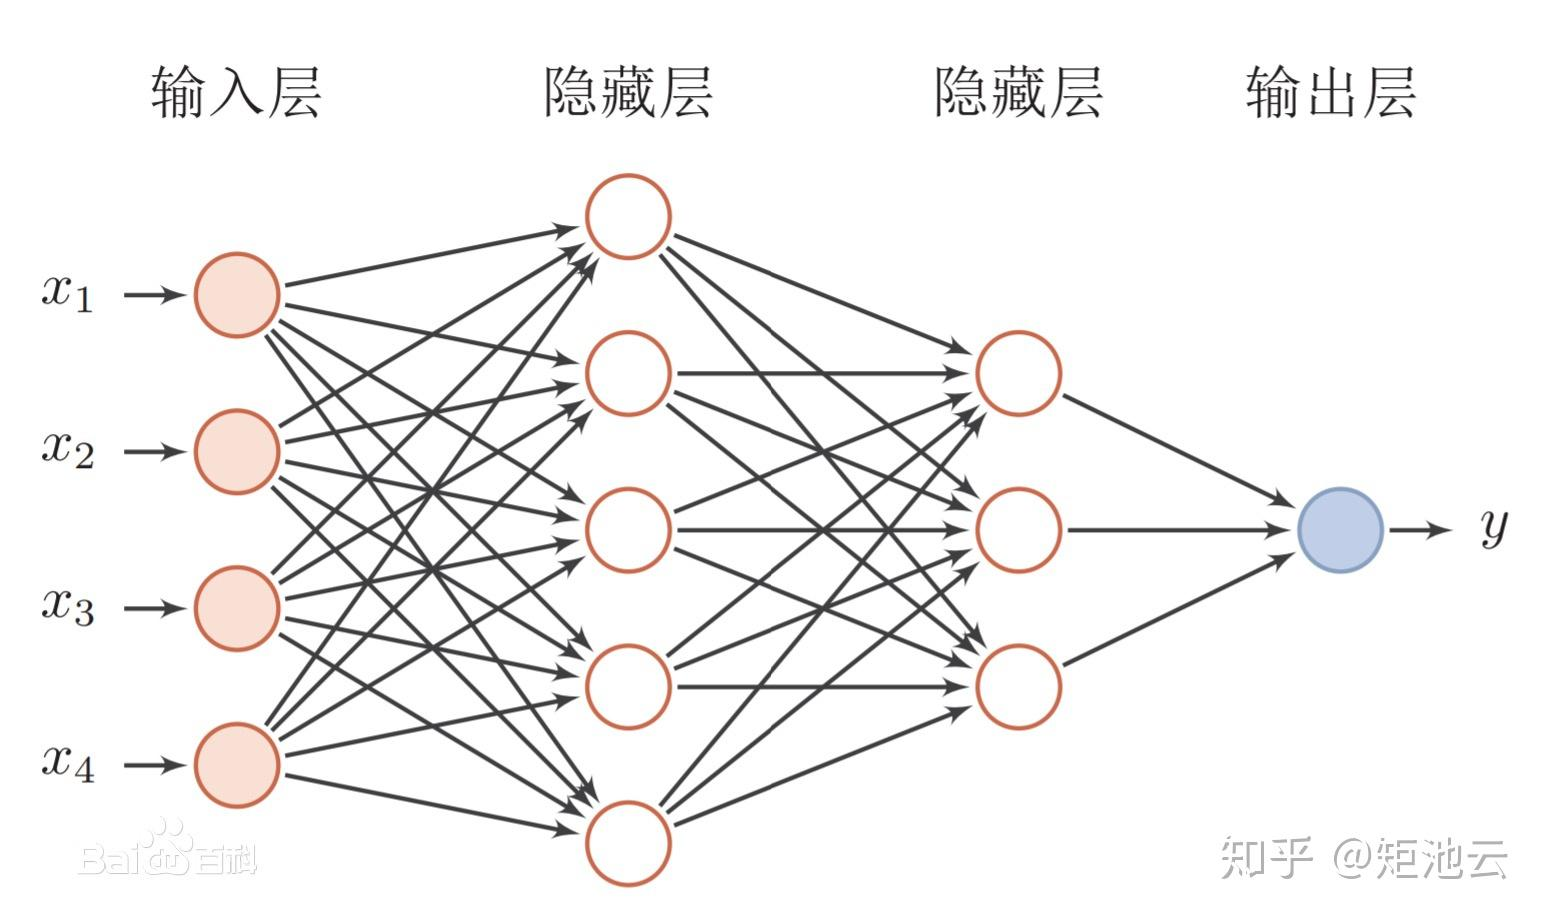
\includegraphics[width=0.8\linewidth]{image/2/神经网络层次结构.jpg}
    \caption{网络层次结构}
    \label{fig:网络层次结构}
\end{figure}


\begin{itemize} 
    \item \textbf{输入层（Input Layer）}：接收原始数据，如图像的像素值、文本的词向量等。
    \item \textbf{隐藏层（Hidden Layers）}：进行特征提取和表示学习，层数越多，网络的“深度”越大。隐藏层的设计直接影响网络的表达能力和学习效果。
    \item \textbf{输出层（Output Layer）}：生成最终的预测结果，如分类标签、回归值等。输出层的结构和激活函数通常根据具体任务进行设计，如分类任务中的 Softmax 层或回归任务中的线性层。
\end{itemize}

此外，现代神经网络中还常见诸如批归一化层（Batch Normalization）、池化层（Pooling Layer）、Dropout 层等特殊层，用于提升网络的稳定性、减少过拟合和加速训练。

\subsubsection{训练过程与优化}

神经网络之所以能够高效地处理和理解复杂的数据，关键在于其训练过程中所展现的“自我调节”能力。在训练阶段，研究人员会向网络提供大量已标注的数据，这些数据相当于神经网络学习的“教材”。网络通过不断地调整内部连接权重和偏置参数，逐步提升对数据的理解与预测能力。当网络的输出结果与实际目标存在偏差时，系统会利用一种称为“反向传播”（Backpropagation）的算法，将这份“误差”逐层传递回每一层的神经元，从而指导网络如何修正权重参数，以最小化预测误差。这一过程类似于教师在指导学生时，指出错误并帮助他们逐步改正。通过多次迭代，网络逐渐在数据中发现潜在的规律，提高了预测的准确性和可靠性。

在这一训练过程中，损失函数（Loss Function）扮演着至关重要的角色。损失函数用于量化模型预测值与真实值之间的差距，为网络的优化提供明确的方向。选择合适的损失函数能够显著影响模型的训练效果和最终性能。不同类型的任务通常会选择不同的损失函数。例如，回归任务常用均方误差（Mean Squared Error, MSE）来衡量预测值与真实值的偏离程度，而分类任务则多采用交叉熵损失（Cross-Entropy Loss），特别是在多分类问题中，通过度量预测概率分布与真实分布之间的差异来优化模型性能。此外，在度量学习和孪生网络等应用中，对比损失（Contrastive Loss）被用于衡量样本对之间的相似度，从而帮助模型更好地捕捉数据中的细微差别。

为了有效地最小化损失函数，优化算法（Optimization Algorithms）被广泛应用于神经网络的训练过程中。最基础的优化方法是梯度下降（Gradient Descent），通过计算损失函数相对于每个参数的梯度，按梯度方向更新参数，以逐步逼近最优解。然而，梯度下降在处理大规模数据集时可能会面临计算效率低下的问题，因此随机梯度下降（Stochastic Gradient Descent, SGD）应运而生。SGD 每次仅使用一个样本或一个小批量样本来计算梯度，从而大幅提升了训练速度，并且在某些情况下还能改善模型的泛化能力。进一步地，动量法（Momentum）在 SGD 的基础上引入了动量项，通过累积过去梯度的指数加权平均，帮助模型加速收敛并减少震荡现象。此外，自适应学习率方法（如 Adam、RMSprop）能够根据参数的历史梯度动态调整学习率，进一步提升训练效率和稳定性。其中，Adam（Adaptive Moment Estimation）结合了动量法和 RMSprop 的优点，成为当前最常用的优化算法之一。

仅有有效的损失函数和优化算法并不足以保证模型的良好性能。神经网络在训练过程中往往会面临过拟合的问题，即模型在训练数据上表现良好，但在未见过的数据上表现较差。为了解决这一问题，正则化（Regularization）技术被引入，以限制模型的复杂度，提高其泛化能力。常见的正则化方法包括L1/L2 正则化，通过在损失函数中加入参数的 L1 或 L2 范数，限制模型权重的大小，防止模型过于复杂；Dropout则是在训练过程中随机忽略部分神经元，减少神经元之间的依赖关系，从而提升模型的鲁棒性；而早停（Early Stopping）则是在验证集性能不再提升时提前停止训练，防止模型在训练数据上过度拟合。尽管神经网络具备强大的学习能力，但在训练过程中仍然面临诸多挑战。其中，梯度消失与梯度爆炸是深层网络中常见的问题，梯度在反向传播过程中可能会逐渐减小（梯度消失）或增大（梯度爆炸），导致网络难以有效训练。为了解决这一问题，研究者们提出了多种方法，包括使用合适的激活函数（如 ReLU）、优化初始化方法（如 He 初始化）以及采用梯度裁剪（Gradient Clipping）等技术来缓解这一问题。此外，深度神经网络通常需要大量的计算资源，这对硬件设备提出了更高的要求。解决这一问题的方法包括部署在 GPU/TPU 上并行加速、应用模型压缩技术（如剪枝、量化）以及采用分布式训练等手段，以降低计算资源的消耗和训练时间。

另一个重要的挑战是模型的解释性差。深度学习模型通常被视为“黑箱”，难以解释其内部工作机制。这在一些需要高可解释性的应用场景中（如医疗诊断、金融风控等）带来了挑战。为了解决这一问题，研究者们开发了多种可解释性技术，如LIME（Local Interpretable Model-agnostic Explanations）和SHAP（SHapley Additive exPlanations），以及尝试设计可解释的模型架构，如将决策树与神经网络结合，以提高深度学习模型的透明度和可信度。

综上所述，神经网络的训练过程就像一场复杂的学习旅程，我们需要高质量的数据作为基础，通过损失函数和优化算法不断调整模型参数，同时运用正则化技术来防止过拟合。在这个过程中，尽管会遇到梯度消失、过拟合、计算资源需求高和模型解释性差等挑战，但通过不断优化训练方法和引入先进技术手段，神经网络在处理复杂任务时的表现得到了显著提升，推动了深度学习技术在各个领域的广泛应用。这不仅展示了神经网络强大的学习和适应能力，也为未来人工智能的发展奠定了坚实的基础。
    
\subsection{神经网络的分类}

了解了神经网络的基本工作原理后，您可能会好奇：在如此灵活的架构中，是否存在不同的“流派”或专精方向？事实上，深度学习领域已经发展出了多种适应不同任务和数据类型的神经网络架构，每一种都有其独特的优势。

神经网络的多样化发展使得它们能够在不同的应用场景中发挥最佳性能。例如，前馈神经网络（Feedforward Neural Network, FNN）作为最基础的深度学习架构，结构简单且直观，适用于基本的分类和回归任务。然而，由于缺乏记忆机制和层次结构，FNN 在处理需要上下文信息或时间序列数据的任务时表现有限。

相比之下，卷积神经网络（Convolutional Neural Network, CNN）则被广泛应用于图像和视频处理。通过卷积层自动提取图像中的关键特征，如边缘、纹理和形状，CNN 极大地提升了计算机的视觉处理能力。例如，在自动驾驶汽车中，CNN 被用于行人检测和交通标志识别，从而提高车辆的安全性和导航能力。典型的 CNN 架构包括 LeNet、AlexNet、VGG 和 ResNet 等，每种架构在深度和复杂度上有所不同，以适应不同的应用需求。

与 CNN 不同，循环神经网络（Recurrent Neural Network, RNN）及其变种（如 LSTM 和 GRU）专注于处理顺序数据，如时间序列、文本或语音。RNN 能够保持记忆，理解序列中前后信息的关联性，因此在自然语言处理任务中被广泛应用于语言模型和机器翻译，能够捕捉句子中的上下文关系。LSTM（长短期记忆）和 GRU（门控循环单元）通过引入门控机制，解决了传统 RNN 在长序列学习中的梯度消失问题，使其在处理长依赖关系时更加高效。

生成对抗网络（Generative Adversarial Network, GAN）则是一种极具创造力的网络架构，由生成器和判别器组成。生成器负责生成新数据，判别器则负责判断数据是否真实。两者在训练过程中相互竞争，通过这种对抗的方式，GAN 能够生成非常逼真的图像、音频甚至艺术作品。例如，GAN 被用于生成高分辨率的人脸图像和艺术风格转换，已经在图像生成、视频制作和数据增强等领域取得了惊人的成果。

图神经网络（Graph Neural Network, GNN）专门用于处理图结构数据，如社交网络和分子结构。它能够捕捉节点之间的复杂关系和图的整体结构，因此在社交网络分析、社区检测和推荐系统中表现出色。此外，在化学和生物领域，GNN 被用于预测分子的性质和药物发现，显示出其在非欧几里得结构数据处理方面的强大适应性。作为 GNN 的具体实现，图卷积网络（Graph Convolutional Networks, GCN）、GraphSAGE 和图注意力网络（Graph Attention Networks, GAT）等进一步丰富了图神经网络的应用和性能。

自编码器（Autoencoder）是一种用于无监督学习和特征降维的网络架构。它由编码器和解码器组成，编码器将输入数据压缩为低维表示，解码器则将其重构回原始数据。例如，自编码器被用于图像去噪和异常检测，通过学习数据的低维表示，能够有效地识别和修复数据中的噪声或异常。变分自编码器（Variational Autoencoder, VAE）是自编码器的一种变体，通过引入概率生成模型，实现更加灵活和有意义的潜在空间表示。

近年来，Transformer 网络凭借其“注意力机制”（Attention Mechanism）在自然语言处理领域取得了巨大成功。与 RNN 不同，Transformer 能够并行处理序列数据，显著提升了训练效率和模型性能。Transformer 及其变种（如 BERT、GPT）在文本生成、机器翻译和问答系统等任务中表现卓越，其自注意力机制能够有效捕捉长距离依赖关系，成为当前深度学习研究的热点。除了 Transformer，注意力机制还被广泛应用于其他神经网络架构，如 Attention RNN 和 Self-Attention 等，进一步增强了模型的表达能力和灵活性。

胶囊网络（Capsule Networks）是另一种较新的神经网络架构，旨在更好地捕捉空间层次关系，特别是在计算机视觉领域有一定的应用。胶囊网络通过“胶囊”这一组神经元来表示实体及其属性，能够更有效地处理对象的姿态、位置和变形等信息，从而提升图像识别的准确性和鲁棒性。

自监督学习模型近年来成为一个重要方向，旨在通过利用未标注的数据进行预训练，从而提升模型在下游任务中的性能。自监督学习通过设计预训练任务（如掩码语言模型、对比学习等）使模型能够学习数据的内在结构和表示，广泛应用于自然语言处理、计算机视觉和多模态学习等领域。

强化学习中的神经网络也是深度学习的重要组成部分。尽管强化学习更多是一个学习范式，但也涉及到特定的神经网络架构，如深度 Q 网络（Deep Q-Networks, DQN）和策略网络（Policy Networks）等。这些网络通过与环境的交互不断优化策略，使得强化学习在游戏、机器人控制和决策制定等领域取得了显著成果。

稀疏神经网络（Sparse Neural Networks）通过引入稀疏连接或稀疏激活，提高模型的效率和可解释性。稀疏神经网络不仅减少了计算资源的消耗，还能够在一定程度上缓解过拟合问题，提升模型的泛化能力。这类网络在资源受限的设备上具有广泛的应用前景，如移动设备和嵌入式系统。

混合模型（Hybrid Models）结合了多种神经网络架构的优势，以应对更加复杂的任务需求。例如，将 CNN 与 RNN 结合用于视频分析，利用 CNN 提取空间特征，RNN 捕捉时间依赖关系；或是将 GAN 与 VAE 结合，用于更稳定和高质量的数据生成。这些混合模型在复杂任务中展现出了强大的能力，推动了深度学习技术的多样化应用。

神经网络的多样化发展不仅在理论上丰富了深度学习的内涵，也在实际应用中展示了其广泛的适用性和强大的性能。随着技术的不断进步，未来将会涌现出更多创新的网络架构，进一步拓展深度学习在各个领域的应用边界。



\subsection{深度学习的优点与挑战}

深度学习作为一种强大的机器学习方法，具有许多显著的优势，但同时也面临一些挑战, 如表\ref{tab:pros-cons}所示。
\begin{longtable}{|>{\RaggedRight}p{0.45\textwidth}|>{\RaggedRight}p{0.45\textwidth}|}
\caption{深度学习：优点与挑战并列表} \label{tab:pros-cons} \\
\toprule
\textbf{优点} & \textbf{挑战} \\
\midrule
\endfirsthead

\multicolumn{2}{c}%
{{\bfseries 表 \thetable\ 续}} \\
\toprule
\textbf{优点} & \textbf{挑战} \\
\midrule
\endhead

\midrule \multicolumn{2}{r}{{续下页}} \\
\endfoot

\bottomrule
\endlastfoot

\textbf{自动特征提取}：深度学习能够自动从原始数据中提取有用的特征，减少对领域知识和手工特征工程的依赖。 &
\textbf{数据需求量大}：深度模型往往需要大量且高质量的训练数据，在某些专业领域数据获取和标注十分困难。 \\
\textbf{处理高维数据的能力}：通过多层抽象结构，能在图像、视频、文本等复杂场景中捕捉丰富的隐含模式。 &
\textbf{计算资源消耗高}：网络训练需要大量计算和存储资源，在移动端或嵌入式设备中部署需模型压缩与优化。 \\
\textbf{强大的泛化能力}：若训练数据充足且正则化得当，模型可在未见过的数据上表现出色。 &
\textbf{模型解释性差}：深度神经网络被视为“黑箱”，难以追溯内部决策逻辑，给高可解释性应用场景带来挑战。 \\
\textbf{可扩展性}：可通过增加网络深度或参数规模，以及分布式训练和硬件加速，处理更大规模、更复杂的任务。 &
\textbf{过拟合风险}：模型参数众多，易在训练数据上记忆过度。需采用正则化、早停或数据增强等手段来缓解。 \\
\textbf{广泛的应用领域}：在计算机视觉、自然语言处理、语音识别、推荐系统、金融分析、医疗等领域取得突破。 &
\textbf{对抗攻击脆弱性}：少量对输入的微扰即可迷惑模型，在自动驾驶、医疗诊断等关键领域需额外防护机制。 \\

\end{longtable}





尽管面临诸多挑战，随着研究的不断深入和技术的进步，许多问题正在逐步得到解决，深度学习的应用前景依然广阔。

\subsection{深度学习的训练技巧与优化方法}

为了提升深度学习模型的性能和训练效率，研究者们开发了许多训练技巧和优化方法。这些方法不仅帮助模型更快地收敛，还能提高其泛化能力和稳定性，从而在各种复杂任务中取得更好的表现。

\subsubsection{学习率调整}

学习率是控制模型参数更新步伐的重要超参数。合适的学习率能够加快训练速度并确保模型收敛到全局最优或局部最优解。选择合适的学习率策略对于有效训练深度学习模型至关重要。

一种常见的调整方法是学习率衰减。随着训练的进行，逐步降低学习率可以帮助模型在接近最优解时进行更细致的调整。比如，在训练的初期使用较高的学习率，可以快速接近最优区域；而在训练后期逐步减小学习率，则有助于模型稳定地收敛，避免在最优解附近来回震荡。常见的衰减策略包括阶梯衰减、指数衰减和余弦衰减，每种策略都有其独特的应用场景和效果。

除了学习率衰减，自适应学习率算法如Adam和RMSprop也被广泛应用。这些算法能够根据参数的历史梯度动态调整每个参数的学习率，从而提高训练效率和稳定性。例如，Adam结合了动量法和RMSprop的优点，不仅加快了收敛速度，还能够在处理稀疏梯度和非平稳目标时表现出色。

此外，循环学习率（Cyclical Learning Rates）是一种较为新颖的方法，通过在训练过程中周期性地增加和减少学习率，帮助模型跳出局部最优解，探索更广阔的参数空间。这种方法不仅加速了训练过程，还能在一定程度上提升模型的泛化能力，使其在面对未见过的数据时表现得更加稳健。

通过合理调整学习率，深度学习模型能够更高效地学习数据中的复杂模式，提升最终的预测准确性和模型的整体性能。

\subsubsection{批归一化（Batch Normalization）}

批归一化是一种在神经网络训练中广泛应用的技术，旨在加速训练过程并提高模型的稳定性。其主要作用是将每一层的输入标准化，使其具有零均值和单位方差，从而缓解内部协变量偏移（Internal Covariate Shift）的问题。内部协变量偏移指的是每一层网络的输入分布在训练过程中不断变化，这会导致训练过程变得不稳定且收敛速度较慢。

通过批归一化，网络的每一层在训练过程中都能保持相对稳定的输入分布，允许使用更高的学习率，加快收敛速度。此外，批归一化在一定程度上起到了正则化的作用，减少了过拟合的风险。这意味着即使在没有其他正则化手段的情况下，模型的泛化能力也会有所提升。

具体而言，批归一化通过对每个小批量的数据进行标准化处理，然后再应用缩放和平移参数，使得每一层的输出既能保持稳定，又能保留必要的表达能力。这一过程不仅提高了训练的效率，还使得模型在面对不同的数据分布时表现得更加鲁棒。

在实际应用中，批归一化已成为深度神经网络架构中的标准组件，被广泛应用于卷积神经网络、循环神经网络等各种类型的网络中。它不仅提升了模型的训练速度，还在很大程度上改善了模型的最终性能，使得训练过程更加顺畅和高效。

\subsubsection{数据增强（Data Augmentation）}

数据增强是一种通过对训练数据进行随机变换（如旋转、翻转、缩放、裁剪等），生成新的训练样本的方法。其主要目的是增加数据的多样性，从而提升模型的泛化能力，减少过拟合风险。特别是在图像处理任务中，数据增强技术极为重要，因为它能够模拟现实世界中的各种变换和噪声，使得模型在面对未见过的样本时依然能够保持良好的表现。例如，在图像分类任务中，原始图像经过随机旋转、翻转或裁剪后，仍然保留了类别的主要特征，从而使模型能够学习到更加鲁棒的特征表示。这不仅扩展了训练数据的规模，还帮助模型更好地适应不同的应用场景。此外，数据增强还可以通过颜色变换、添加噪声等方式，进一步丰富训练数据的多样性。

除了图像处理，数据增强技术也广泛应用于自然语言处理和语音识别等领域。例如，在文本处理中，可以通过同义词替换、随机插入或删除词汇等方法来生成新的训练样本；在语音识别中，可以通过添加背景噪声或改变语速来增强数据集。这些方法不仅丰富了训练数据，还能有效提升模型在真实环境中的表现。

数据增强不仅能够提高模型的泛化能力，还能在一定程度上提高模型对噪声和变形的鲁棒性，使得模型在实际应用中更加可靠和稳定。随着研究的深入，更多高级的数据增强方法如混合增强（Mixup）、马赛克增强（Mosaic）等也被提出，进一步提升了数据增强的效果和应用范围。

\subsubsection{迁移学习（Transfer Learning）}

迁移学习通过将一个任务中学到的知识应用到另一个相关任务中，显著减少了新任务所需的训练数据量和训练时间。常见的迁移学习方法包括使用预训练模型作为特征提取器，或在预训练模型的基础上进行微调（Fine-Tuning）。例如，在计算机视觉领域，研究者们常使用在ImageNet上预训练的ResNet作为基础模型，然后在特定的分类任务上进行微调。这种方法不仅能够快速提升模型的性能，还能显著减少训练所需的计算资源和时间。预训练模型已经在大规模数据集上学到了丰富的特征表示，这些特征可以有效地迁移到其他相关任务中，从而提升新任务的表现。

同样，在自然语言处理领域，预训练的Transformer模型如BERT和GPT也被广泛应用于各种下游任务，如文本分类、问答系统和文本生成等。通过迁移学习，模型能够利用在大规模文本数据上学到的语言知识，快速适应新的任务需求，提高任务的完成效果。

迁移学习不仅提高了模型的性能，还大幅降低了训练的难度和成本，使得深度学习技术在资源受限的环境中也能得到有效应用。此外，迁移学习还能够帮助模型在面对数据稀缺或标注困难的任务时，依然能够保持良好的表现，进一步扩展了深度学习的应用范围。

随着研究的不断深入，迁移学习的方法和策略也在不断演化，如多任务学习（Multi-Task Learning）、跨域迁移（Domain Adaptation）等，进一步提升了迁移学习的效果和适用性。未来，迁移学习有望在更多领域发挥重要作用，推动深度学习技术的广泛应用和发展。

\subsubsection{模型压缩与加速}

深度学习模型通常具有大量的参数和高计算需求，这在实际应用中，尤其是在资源受限的环境中（如移动设备和嵌入式系统），成为一大挑战。为了在这些环境中高效部署深度学习模型，研究者们开发了多种模型压缩与加速技术。

剪枝（Pruning）是通过移除不重要的神经元或连接，减少模型的规模和计算量的一种方法。剪枝技术能够显著降低模型的参数数量和计算复杂度，从而提高推断速度。例如，通过权重剪枝，可以去除那些权重值较小且对最终输出影响不大的连接，保持模型性能的同时，减少计算资源的消耗。此外，结构化剪枝方法通过移除整个通道或层，进一步优化模型的结构，使其更适合硬件加速。

量化（Quantization）则是将模型参数从高精度（如32位浮点数）降低到低精度（如8位整数），以减少存储需求和计算复杂度。量化技术不仅能够显著减少模型的存储空间，还能提升计算效率，特别适用于移动端和嵌入式设备的部署。近年来，研究者们提出了多种量化方法，如对称量化、非对称量化和动态量化，以适应不同的应用需求。例如，动态量化在推断阶段根据输入数据动态调整量化参数，进一步提高了模型的灵活性和性能。

知识蒸馏（Knowledge Distillation）是一种通过训练一个小型“学生”模型模仿大型“教师”模型的行为，保持性能的同时减少模型规模的方法。知识蒸馏技术能够将教师模型中学到的知识迁移到学生模型中，使得学生模型在保持高准确度的同时，具备更轻量化和高效的特点。这种方法不仅适用于模型压缩，还能提升小模型在特定任务上的表现。通过软标签（soft targets）或中间层特征的匹配，学生模型能够更好地捕捉教师模型的知识，提高自身的学习能力和泛化性能。

除了上述方法，模型压缩与加速还包括低秩分解（Low-Rank Decomposition）、网络剪枝（Network Pruning）和参数共享（Parameter Sharing）等技术。这些方法通过不同的策略优化模型结构和参数分布，使得模型在保持性能的同时，减少了计算资源的消耗和存储需求。

通过这些模型压缩与加速方法，深度学习模型能够在资源受限的环境中高效运行，拓展了其在实际应用中的适用范围。这不仅提高了深度学习模型的实用性，还使得深度学习技术能够在更多领域得到广泛应用，如移动设备、物联网、边缘计算等，进一步推动了人工智能技术的普及与发展。

综上所述，深度学习的训练技巧与优化方法在提升模型性能、加速训练过程和提高模型泛化能力方面发挥了重要作用。通过合理地应用学习率调整、批归一化、数据增强、迁移学习以及模型压缩与加速等技术，研究者们能够设计出高效、稳定且具有强大表现力的深度学习模型，从而推动深度学习技术在各个领域的广泛应用与发展。

\section{总结}
通过本章对人工智能、机器学习和深度学习三大领域的系统阐述，我们能够更全面地理解当前智能系统所依赖的技术框架与方法演进逻辑，同时也对AI从早期符号推理到数据驱动，再到复杂神经网络的发展历程有了更深刻的认识。

在 2.1 节，我们首先从宏观层面探讨了人工智能（AI）的广泛内涵与核心目标：让机器能够感知、推理、决策并不断学习，从而在医疗、金融、交通等诸多领域中扮演“智慧助手”乃至“决策者”的角色。然而，早期的规则和符号系统在面对复杂、不确定性高的问题时往往力不从心，因而发展出基于数据驱动的机器学习（ML）方法，让计算机通过海量数据自行发现其中的规律和模式。进一步地，为了在海量、复杂、多维度的数据中实现更高层次的抽象与模式捕捉，深度学习（DL）依托多层神经网络的结构优势，取得了跨越式成果，成为当前推动AI进化的核心引擎。

在 2.2 节 中，我们聚焦于机器学习本身的概念、原理与实践。与传统编程需要显式地写出所有规则不同，机器学习让计算机“观摩”并分析大规模数据，自动生成相应的判断与预测逻辑，因而极大提升了适应力与扩展性。我们通过“烘焙学徒”的类比理解了机器学习的基本过程——从数据采集与特征提取，到模型训练与评估，再到反复的验证与优化，最终使模型具备在新环境中自如应对的能力。同时，机器学习根据任务的不同可分为监督学习、无监督学习、强化学习和迁移学习等分支，分别适用于不同的数据形态和应用场景。在各种模型和算法的基础上，机器学习为自然语言处理、图像识别、自动驾驶等领域提供了灵活而高效的方法支撑。

进入 2.3 节，我们对深度学习的核心原理与神经网络架构进行了更加深入的讨论。深度学习之所以被称为“深度”，正是因为其通过多层的神经元网络，能够在庞大且复杂的数据中进行层次化的表征学习，从而在图像、语音、文本等任务中挖掘到更抽象、更富表现力的特征。卷积神经网络（CNN）在计算机视觉、循环神经网络（RNN）及其变体在自然语言处理与时间序列分析、生成对抗网络（GAN）在图像合成与数据增强等方面的成功，皆证明了深度学习在高维数据建模上的优势。不仅如此，随着硬件性能和大数据资源的不断发展，深度学习在工程上的瓶颈逐渐被突破，各种分布式训练、模型压缩与优化技巧也进一步拓展了其在移动端、嵌入式设备等资源受限环境的应用。

综合而言，本章从宏观（2.1）到微观（2.2、2.3），一步步带领我们了解了现代人工智能技术体系的基础结构：AI 提供了整体目标与愿景，机器学习通过数据驱动的方式赋予系统自我学习的能力，而深度学习在更深层次的网络结构上实现了对复杂数据的高效建模与自动特征提取，显著提升了AI解决复杂问题的能力。它们三者之间的层级联系，也为读者理解当代智能系统的全貌提供了有效的脉络。

在接下来的学习或应用过程中，我们还将更加深入地探讨深度学习在特定领域和实际场景中的部署与优化，包括网络结构设计、训练过程中的技术细节、模型评估与安全性挑战等方面。通过对这些内容的系统掌握，读者将能够更全面地把握人工智能的前沿动态，并为各行各业的创新与实践提供有力的技术支持。


\section{第二章复习题}

\textbf{选择题}

\begin{enumerate}
  \item \textbf{关于人工智能（AI）、机器学习（ML）与深度学习（DL）的关系，下列说法正确的是：}
  \begin{enumerate}[A.]
    \item 机器学习是人工智能的一个子领域，深度学习又是机器学习的一个分支
    \item 人工智能的概念范围最小，深度学习范围最大
    \item 深度学习和机器学习完全独立，二者并无联系
    \item 人工智能中最主要的实现手段是符号推理，机器学习和深度学习并不重要
  \end{enumerate}

  \textbf{参考答案：} A

  \textbf{解析：}  
  \textbf{A}：AI 的范围最广，ML 是其中的数据驱动方法，而 DL 则是 ML 的子集，故“AI $\supseteq$ ML $\supseteq$ DL”最为准确。  
  \textbf{B} 说法相反； \textbf{C} 认为 DL 与 ML 毫无关联，错误； \textbf{D} 过度强调符号推理，忽视了机器学习和深度学习在当前 AI 中的核心地位。

  \item \textbf{在机器学习（ML）中，以下哪一个过程最能体现“数据驱动”的思想？}
  \begin{enumerate}[A.]
    \item 根据专家经验为模型编写所有可能出现的规则
    \item 为计算机提供大量标注过的样本，用来训练模型并让其自动学习规律
    \item 在模型部署后，手动修正模型的预测结果
    \item 使用传统编程方式，为所有情况编写 \texttt{if-else} 条件分支
  \end{enumerate}

  \textbf{参考答案：} B

  \textbf{解析：}  
  机器学习的核心在于让模型通过大量\textbf{训练数据}“自动”学习和提炼模式，而非在代码中人工编写规则。A、C、D 都违背了“数据驱动”的理念。

  \item \textbf{以下哪种神经网络结构最适合处理“图像识别”任务？}
  \begin{enumerate}[A.]
    \item 循环神经网络（RNN）
    \item 卷积神经网络（CNN）
    \item 生成对抗网络（GAN）
    \item 前馈神经网络（FNN）
  \end{enumerate}

  \textbf{参考答案：} B

  \textbf{解析：}  
  CNN 通过卷积与池化操作捕捉图像局部特征并减少参数量，最常用于图像与视频处理；RNN 适合序列数据；GAN 属于生成模型；FNN 结构简单，对图像的特征提取能力较弱。

  \item \textbf{下列关于深度学习优点的描述，哪一项是不恰当的？}
  \begin{enumerate}[A.]
    \item 自动特征提取，减少对手工特征工程的依赖
    \item 能够轻松地处理并理解小规模、数据匮乏的场景
    \item 在计算机视觉、自然语言处理等领域取得了突破
    \item 随着网络深度加深，对大规模数据具有出色的表达能力
  \end{enumerate}

  \textbf{参考答案：} B

  \textbf{解析：}  
  深度学习对大规模、优质数据的依赖度很高，在数据不足的场景中往往难以充分发挥优势。A、C、D 均是深度学习的常见优点。

  \item \textbf{在机器学习过程中的“评估阶段”，下列哪项通常不被用作衡量分类模型性能的指标？}
  \begin{enumerate}[A.]
    \item 准确率 (\textit{Accuracy})
    \item 精确率 (\textit{Precision})
    \item 召回率 (\textit{Recall})
    \item 均方误差 (\textit{MSE})
  \end{enumerate}

  \textbf{参考答案：} D

  \textbf{解析：}  
  准确率、精确率与召回率等指标主要衡量\textbf{分类}模型性能；MSE（均方误差）一般用于\textbf{回归}任务衡量预测与真实值的差异。

\end{enumerate}

\textbf{简答题}

\begin{enumerate}
  \item \textbf{简述人工智能、机器学习与深度学习的层次关系。}

  \textbf{参考要点：}
  \begin{itemize}
    \item \textbf{人工智能（AI）：} 范围最广，目标是让机器具备人类般的感知、推理和决策能力，包括符号推理、专家系统、机器学习等多种方法。
    \item \textbf{机器学习（ML）：} AI 的重要分支，通过海量数据训练模型自动发现模式与规律，摆脱人工设定规则。
    \item \textbf{深度学习（DL）：} 机器学习的子领域，基于多层神经网络的强大特征提取与表达能力，尤其适用于高维度和复杂数据。
    \item 三者关系可概括为：\textbf{AI $\supseteq$ ML $\supseteq$ DL}。
  \end{itemize}

  \textbf{简要解析：}
  早期 AI 多依靠符号推理，难以处理复杂场景；ML 用数据驱动的方式扩展了 AI 能力；DL 则在图像、语音、文本等领域取得重大突破，是 ML 的重要发展方向。

  \item \textbf{在机器学习训练流程中，为什么需要进行模型评估和优化？}

  \textbf{参考要点：}
  \begin{itemize}
    \item \textbf{评估目的：} 检验模型对新数据的泛化能力，防止“死记硬背”训练集（过拟合）。
    \item \textbf{评估指标：} 分类任务常见 \textit{Accuracy}、\textit{Precision}、\textit{Recall}、\textit{F1} 分数等；回归任务可用 \textit{MSE}、\textit{MAE} 等。
    \item \textbf{优化过程：} 通过分析评估结果，调参或改进数据预处理，最终提升模型鲁棒性与表现。
  \end{itemize}

  \textbf{简要解析：}
  训练后的模型若不评估，就无法判断是否具有实际应用价值；模型评估帮助我们发现不足并进行针对性调整，从而得到更优的学习效果。

  \item \textbf{简要说明深度学习在数据需求、计算资源、模型可解释性方面面临的挑战。}

  \textbf{参考要点：}
  \begin{itemize}
    \item \textbf{数据需求量大：} 复杂神经网络通常需要海量优质标注数据才能充分训练。
    \item \textbf{计算资源消耗高：} 训练深层网络需 GPU、TPU 等强大硬件，耗时和硬件成本较高。
    \item \textbf{可解释性不足：} 多层神经网络常被视为“黑箱”，难以清晰解释内部决策过程，在高风险场景中存在应用门槛。
  \end{itemize}

  \textbf{简要解析：}
  虽然深度学习在诸多领域成绩斐然，但在数据、算力和可解释性上仍存在瓶颈，学术和工业界正致力于研发模型压缩、可解释性方法等技术。

  \item \textbf{简要对比 CNN（卷积神经网络）与 RNN（循环神经网络）的主要应用场景差异。}

  \textbf{参考要点：}
  \begin{itemize}
    \item \textbf{CNN：} 主要处理图像、视频等\textbf{空间结构}数据，通过卷积操作高效提取局部特征。
    \item \textbf{RNN：} 专注\textbf{序列数据}（如文本、语音），可记忆上下文，实现对时间或顺序相关性较强的任务建模。
  \end{itemize}

  \textbf{简要解析：}
  CNN 擅长平面/空间域；RNN 则针对连续序列（时序）问题更具优势，二者也可结合（如视频理解），充分发挥各自特长。

\end{enumerate}

\textbf{论述题}

\begin{enumerate}
  \item \textbf{结合本章所学，试论述“为什么深度学习被称为推动当代人工智能飞速发展的核心动力”？}

  \textbf{参考要点：}
  \begin{itemize}
    \item \textbf{多层特征表示：} 能在高维度数据中层层抽象提取出丰富特征。
    \item \textbf{自动特征提取：} 减少手工工程依赖，大幅提升精度与效率。
    \item \textbf{关键领域突破：} 在图像、语音、NLP 等方面屡破纪录，带动产业落地。
    \item \textbf{硬件与数据支撑：} GPU、TPU、大规模数据集共同促进深度网络训练发展。
    \item \textbf{创新生态：} Transformer、GAN、Attention 机制等不断涌现，为研究提供新思路。
  \end{itemize}

  \textbf{论述参考解析：}
  深度学习在多层神经网络中通过非线性变换自动学习特征与映射关系，弥补了传统 ML“特征工程”耗时、效用受限的不足。在图像识别、语言理解等现实场景中，它成为推动 AI 快速发展的强大引擎。

  \item \textbf{请分析“机器学习的自适应能力”对传统显式编程方式带来的冲击及优势。}

  \textbf{参考要点：}
  \begin{itemize}
    \item \textbf{传统编程方式：} 需人为编写大量 \texttt{if-else} 规则，维护困难且对复杂情境缺乏弹性。
    \item \textbf{ML 的自适应：} 通过训练数据自动提炼通用规律，遇到新情况可追加数据或更新模型，无需重新编写所有逻辑。
    \item \textbf{应用优势：} 能在高维和动态环境下有效运转，减少人工维护成本和逻辑漏洞。
  \end{itemize}

  \textbf{论述参考解析：}
  机器学习的自动归纳能力极大地降低了编写和维护规则的难度，对需要灵活应对多变场景（如电商推荐、图像识别）的任务而言，ML 具备传统编程无法企及的拓展潜能。

  \item \textbf{结合2.1、2.2、2.3的知识，谈一谈你对未来人工智能发展趋势的看法。}

  \textbf{参考要点（示例）：}
  \begin{itemize}
    \item \textbf{符号推理与数据驱动融合：} AI 或将结合知识图谱、因果推理，提高高层决策能力与可解释性。
    \item \textbf{多模态与跨领域：} 文本、图像、语音、传感器等数据融合，广泛应用于交通、医疗、金融、教育等。
    \item \textbf{大模型与小模型并存：} 通用预训练大模型在云端发挥优势，小型或压缩模型适用于移动端或嵌入式。
    \item \textbf{安全与合规：} 深度学习模型缺乏可解释性，且易受对抗攻击，需要更多研究与监管策略。
  \end{itemize}

  \textbf{论述参考解析：}
  AI 的未来离不开多种技术路径的交互发展；\textbf{深度学习}仍会在大数据、高性能计算浪潮下持续爆发，但对可解释、安全合规、隐私保护等方面的诉求也将成为下一轮创新焦点。

\end{enumerate}

